\documentclass[12pt]{beamer}
\usetheme[navbar=false, bkgimage=false, shadow=true]{Fermi}

\usepackage{graphicx}

\usepackage{amsmath}
\usepackage{xspace}

\newcommand{\gtlike}{\ensuremath{\mathtt{gtlike}}\xspace}
\newcommand{\pointlike}{\ensuremath{\mathtt{pointlike}}\xspace}
\newcommand{\gtobssim}{\ensuremath{\mathtt{gtobssim}}\xspace}
\newcommand{\fermi}{\textit{Fermi}\xspace}

\title{Search for Spatially Extended \fermi-LAT Sources Using Two Years of Data}

\author{Joshua Lande,\\
Stefan Funk,\\
Markus Ackermann}
\date{August 25, 2011}

\begin{document}

\fermititle

\begin{frame}{paper}

  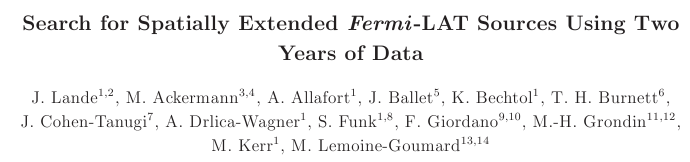
\includegraphics[scale=0.45]{plots/title.png}

  \begin{itemize}
    \item Cat II paper
    \item Target Journal: ApJ
    \item Pub Board: \url{https://www-glast.stanford.edu/cgi-prot/pub_download?id=662}
    \item Internal referees: Marianne Lemoine-Goumard + Johann Cohen-Tanugi (+ unofficially Jean Ballet)
      \begin{itemize}
        \item Thanks for all your help!
      \end{itemize}
    \item Ready for submission
  \end{itemize}
\end{frame}

\begin{frame}{Section 2.1. Modeling Extended Sources in the \texttt{pointlike} Package}
  New method to study spatially-extended {\em Fermi}-LAT sources
  \begin{itemize}
    \item Description of \texttt{pointlike}
    \item Implementation of extended sources
    \item Simultaneously Fit position + extension
    \item speed up likelihood computation
    \item Cross check TS + spectral values using \texttt{gtlike}
  \end{itemize}
\end{frame}


\begin{frame}{Fig. 3+4: False-Detection Rate}
  \begin{columns}
    \column{.5\textwidth} 
    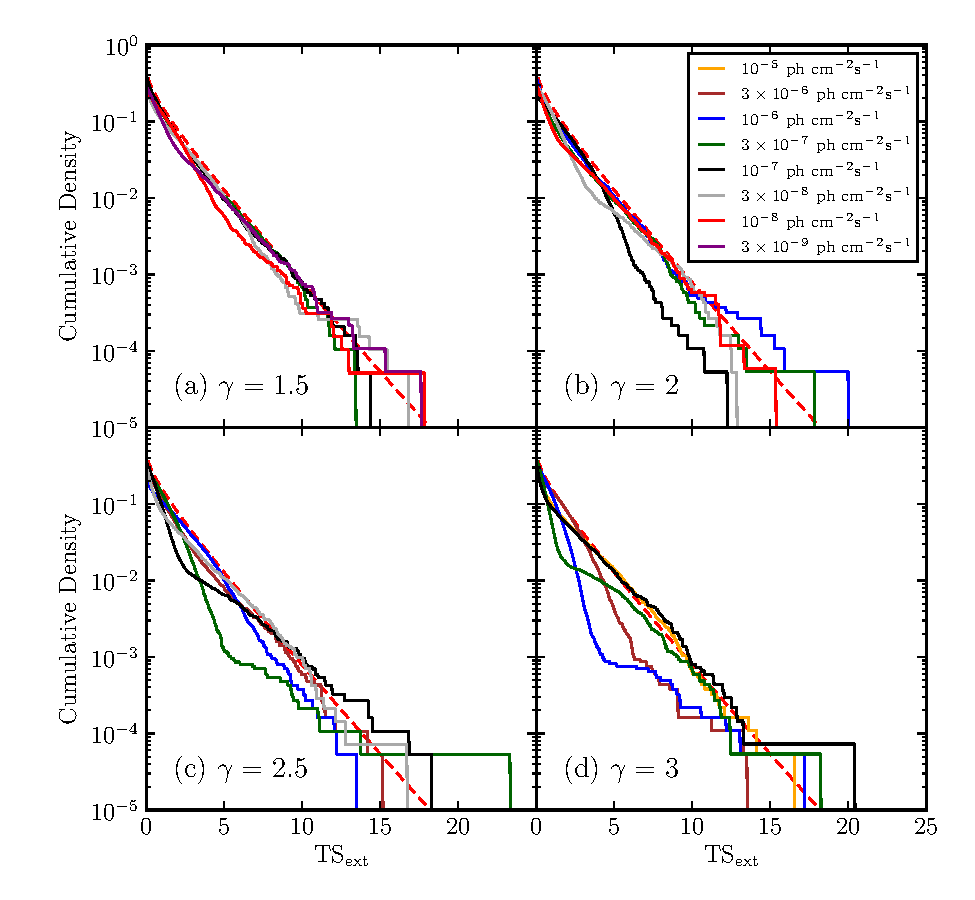
\includegraphics[scale=0.4]{plots/ts_ext_emin_1000_color.pdf}
    \column{.5\textwidth} 
    \begin{itemize}
      \item Simulate point-like sources
      \item Test for extension
      \item Good agreement with Wilk's Theorem
      \item Use $\sqrt{\mathrm{TS}_\mathrm{ext}}$
        as a measure of significance
      \item $\sim 20,000$ Simulations per spectral model!
      \item Test in 1 GeV to 100 GeV + 10 GeV to 100 GeV
        energy range
    \end{itemize}
  \end{columns}
\end{frame}

\begin{frame}{Fig. 5+6+7: Detection Threshold}
  \begin{columns}
    \column{.6\textwidth}
    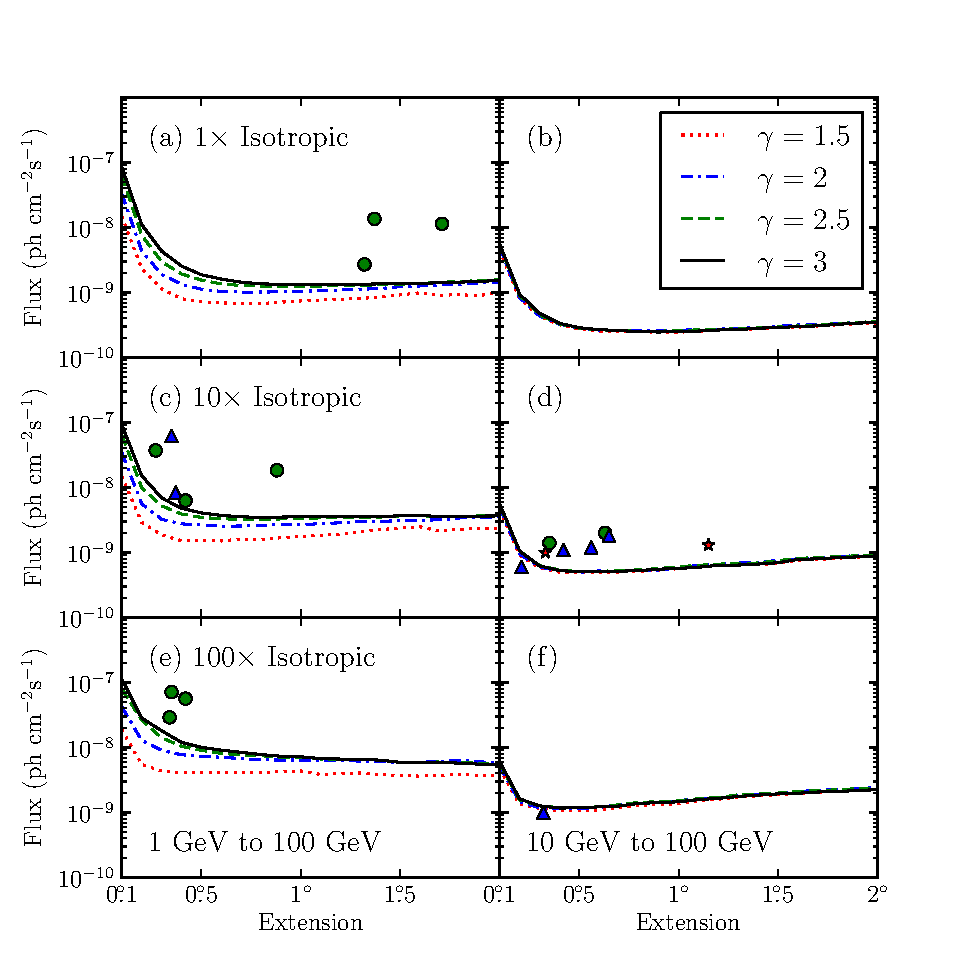
\includegraphics[scale=0.5]{plots/all_sensitivity_color.pdf}
    \column{.4\textwidth}
    \begin{itemize}
      \item Detetion threshold to extension
      \item $\langle\text{TS}_\text{ext}\rangle=16$
      \item Vary spectra, background, energy range
      \item Overlay extended sources
      \item Reference for future publications!
    \end{itemize}
  \end{columns}
\end{frame}

\begin{frame}{Fig. 8+9: Effects of Source Confusion}
  Non-nested model comparison
  \begin{equation*}
    \text{TS}_\text{2pts} = 2 \log(\mathcal{L}_\text{2pts}/\mathcal{L}_\text{ps})
  \end{equation*}

  \begin{columns}
    \column{.6\textwidth}
    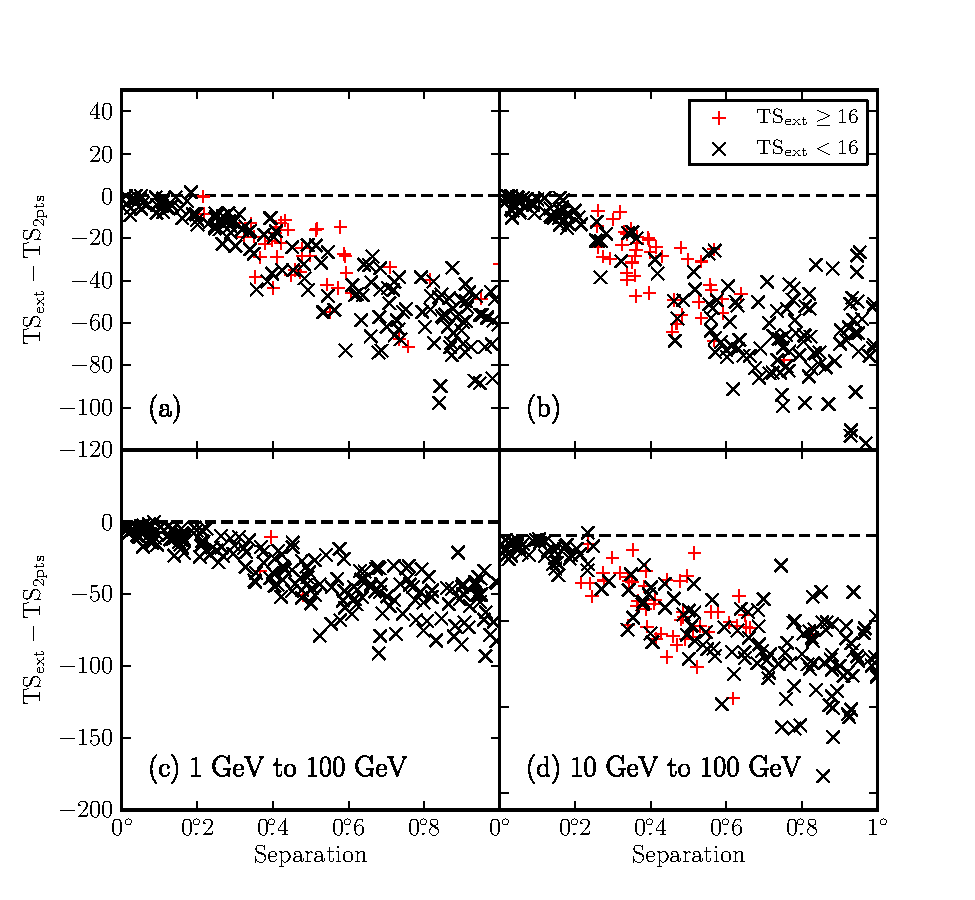
\includegraphics[scale=0.30]{plots/confusion_2pts_plot_color.pdf}

    Simulate extended sources. Fit as point-like sources.

    \column{.4\textwidth}
    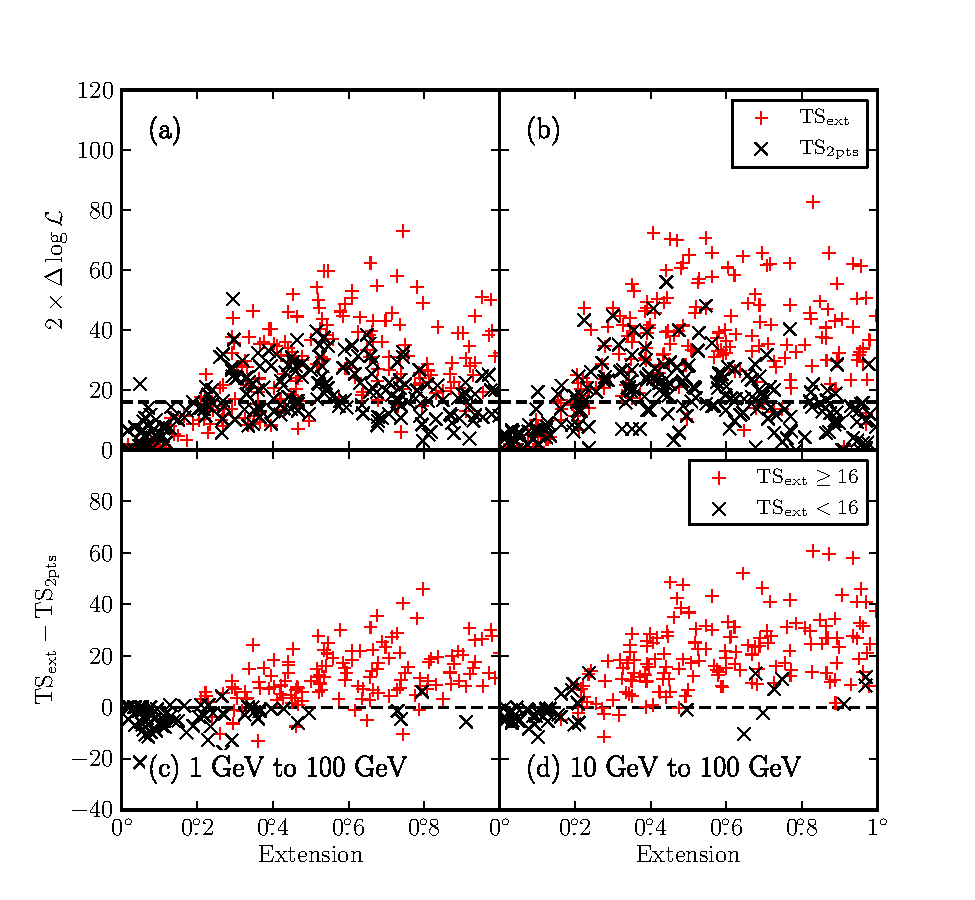
\includegraphics[scale=0.30]{plots/confusion_extended_plot_color.pdf}

    Simulate point-like sources. Fit for extension.
  \end{columns}
\end{frame}


\begin{frame}{Fig. 10: $\text{TS}_\text{ext}$ for 2LAC AGN}
  \begin{columns}
    \column{.6\textwidth}
    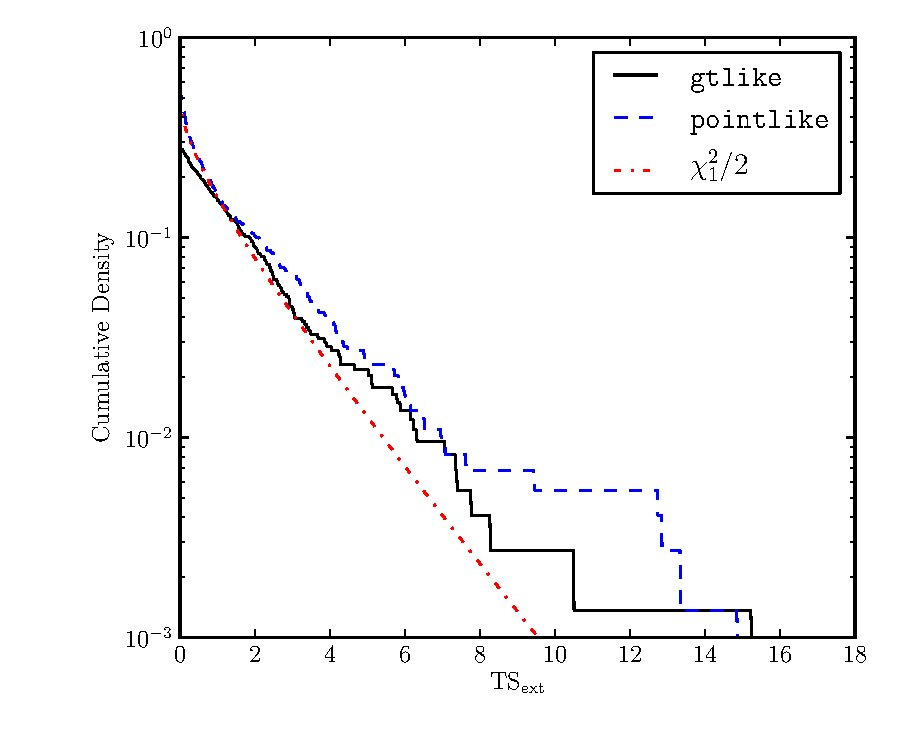
\includegraphics[scale=0.45]{plots/agn_color.pdf}
    \column{.4\textwidth}
    \begin{itemize}
      \item Use point-like AGN to validate extended source analysis
      \item Test clean 2LAC AGN for extension
      \item Don't find AGN to be extended!
    \end{itemize}
  \end{columns}
\end{frame}


\begin{frame}{Section 7: extended sources in 2FGL}
  \begin{columns}
    \column{.6\textwidth}
    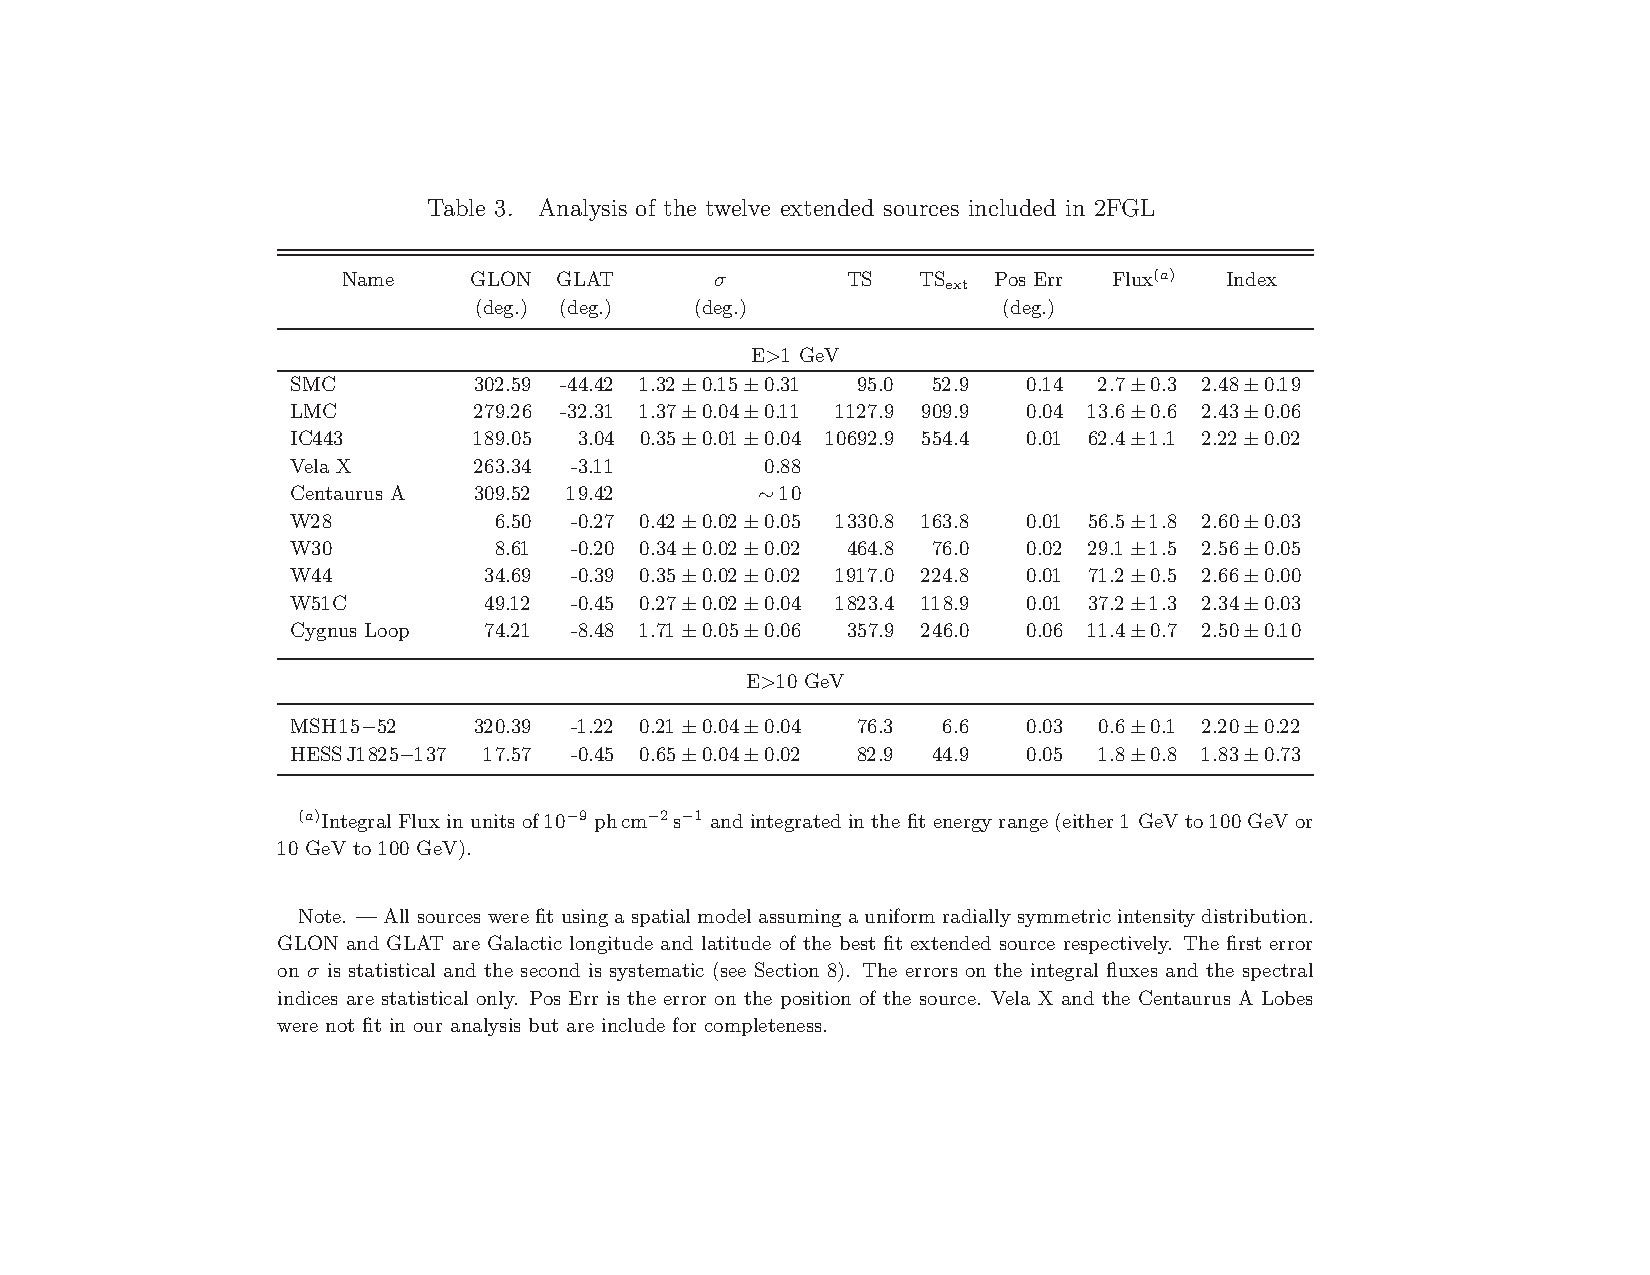
\includegraphics[scale=0.4]{plots/table_reanalysis.pdf}
    \column{.4\textwidth}
    \begin{itemize}
      \item Test 12 extended 2FGL sources for extension
      \item Systematic reanalysis using 2 years of data.
      \item Assume uniform disk
      \item Extended sources are extended!
    \end{itemize}
  \end{columns}
\end{frame}

\begin{frame}{Section 8: Extension Systematics}
  Test systematics due to not knowing PSF
  \begin{itemize}
    \item Compare best fit extension to 
      MC based PSF
    \item Use difference as systematic
    \item Small effect on extension, large effect on statistical 
      significance
    \item Probably too conservative\dots
  \end{itemize}
  Test systematics due to not knowing PSF
  \begin{itemize}
    \item Break up GALPROP diffuse model into multiple components 
    \item Fit each component locally
    \item Tests systematics due to imperfect diffuse modeling
  \end{itemize}
\end{frame}

\begin{frame}{Section 9: Extended Source Search}
  \begin{itemize}
    \item Run a dedicated search 
    \item Find previously-unresolved
      extended 2FGL sources
    \item Search for $E>1$ GeV and $E>10$ GeV
    \item Many difficulties in search, discussed at length in text\dots
    \item Publish only good candidates
  \end{itemize}
\end{frame}

\begin{frame}{Section 10: New extended Sources}
  \begin{columns}
    \column{.65\textwidth}
    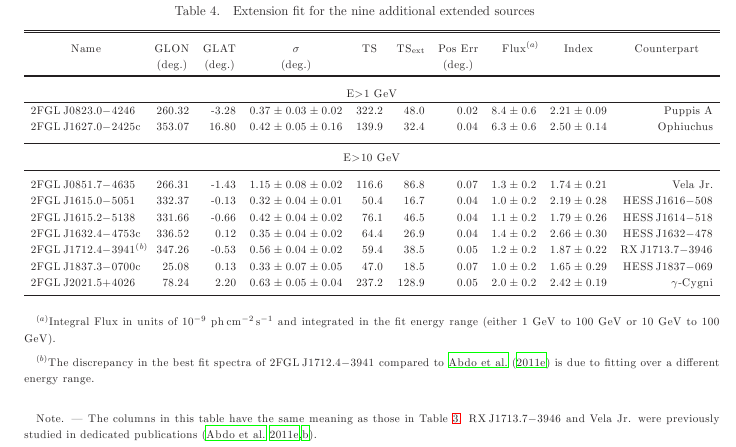
\includegraphics[scale=0.30]{plots/new_extended.png}
    \column{.35\textwidth}
    \begin{itemize}
      \item 6 new extended sources
      \item + RX J1713-3946 \& Vela Jr (not extended in 2FGL)
      \item + 1 source in Ophiuchus region $\rightarrow$ diffuse emission
    \end{itemize}
  \end{columns}
\end{frame}



\begin{frame}{2 Extended SNRs}
  \begin{columns}
    \column{.50\textwidth} 
    Puppis A

    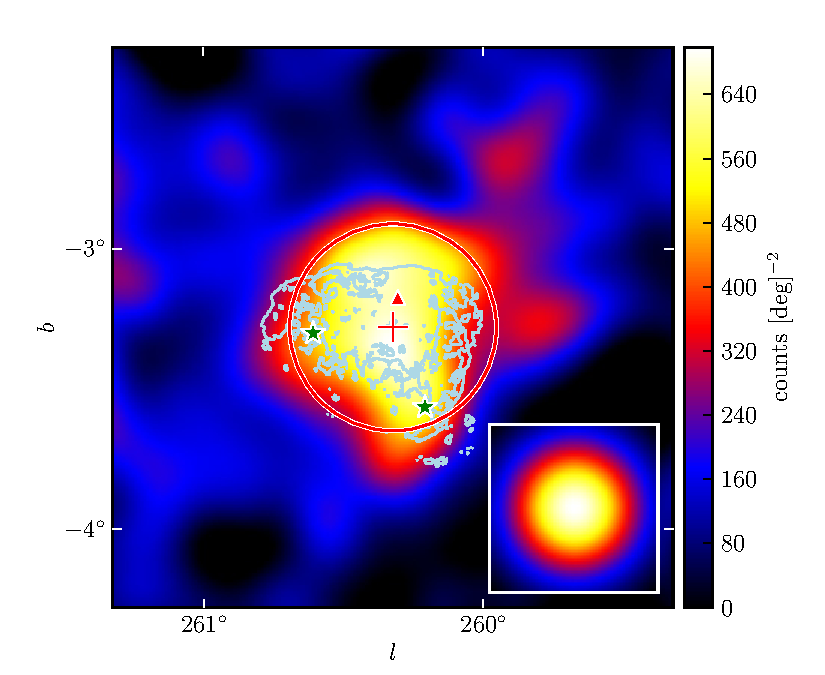
\includegraphics[scale=0.40]{plots/source_Puppis_A_color.pdf}

    \begin{itemize}
      \item X-ray contours
      \item Mid-aged SNR
      \item Not observed to directly interact with molecular
        clouds
      \end{itemize}

    \column{.50\textwidth} 
    $\gamma$-Cygni

    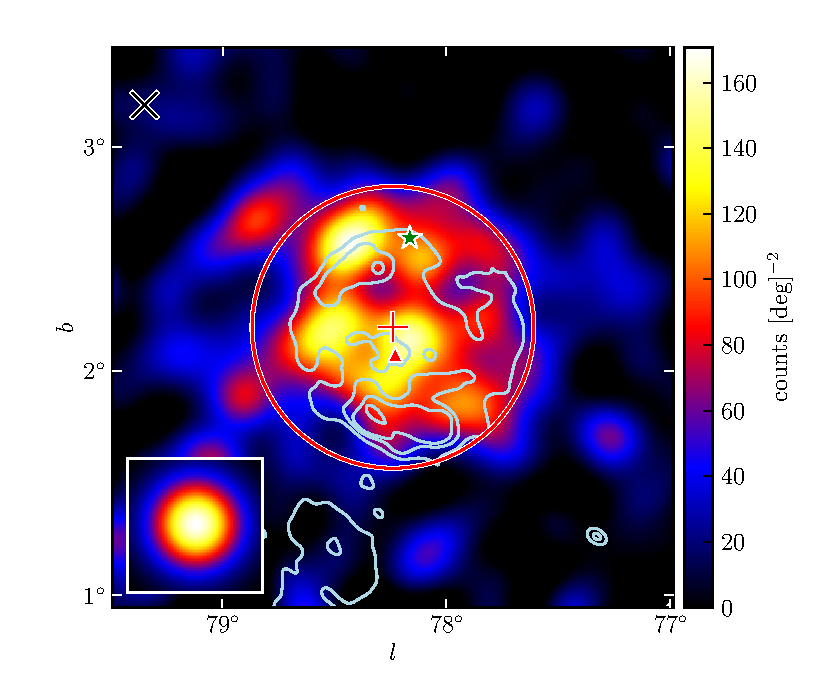
\includegraphics[scale=0.40]{plots/source_Gamma_Cygni_color.pdf}

    \begin{itemize}
      \item Radio contours
      \item SNR interacting with molecular clouds?
      \item Veritas + Milagro detections
      \end{itemize}
  \end{columns}
\end{frame}


\begin{frame}{Two Nearby LAT extended sources}


  \begin{columns}
    \column{.6\textwidth} 
    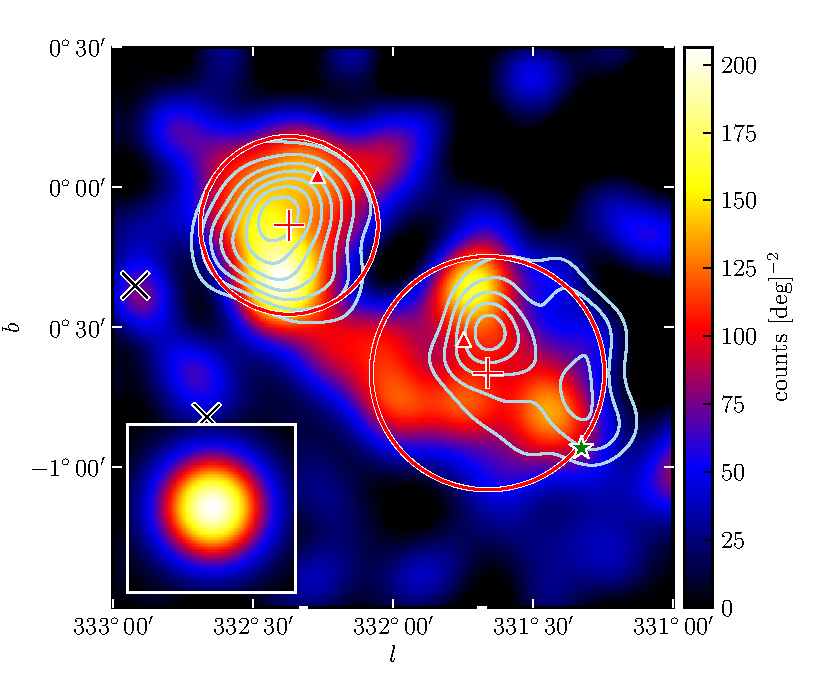
\includegraphics[scale=0.5]{plots/source_HESS_J1614-518_color.pdf}
    \column{.4\textwidth} 
    \begin{itemize}
    \item (left): 
      2FGL\,J1615.0$-$5051
    \item Coincident with HESS\,J1616$-$508
    \item + X-ray pulsar
PSR\,J1617$-$5055 + $\sim 1'$ PWN 
    \item PWN Candidate
    \end{itemize}
  \end{columns}

  \begin{itemize}
    \item (right):
      2FGL\,J1615.2$-$5138 
    \item Coincident with HESS\,J1614$-$518
    \item No other compelling multiwavelenth counterpart
  \end{itemize}
\end{frame}

\begin{frame}{2 More PWN Candidate}


  \begin{columns}
    \column{.45\textwidth} 

2FGL\,J1632.4$-$4753c 

    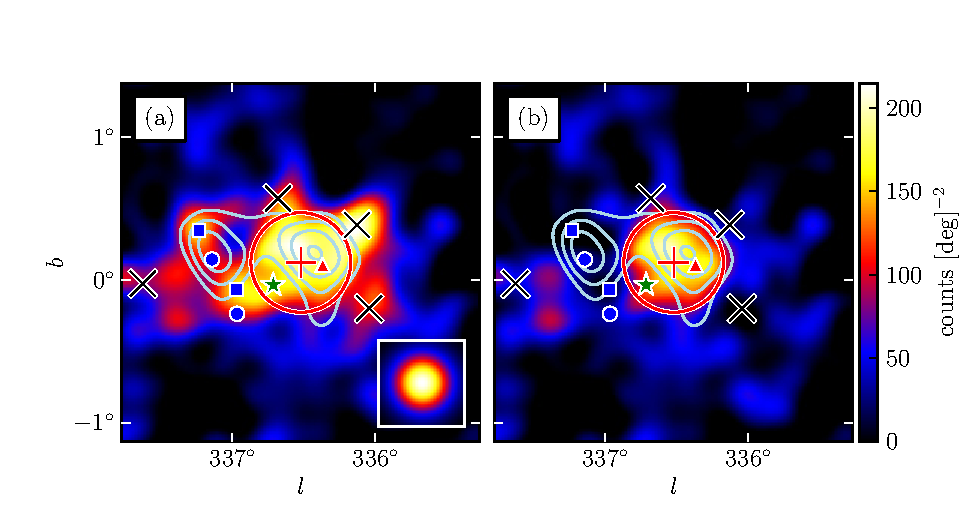
\includegraphics[scale=0.3]{plots/source_HESS_J1632-478_color.pdf}

    \begin{itemize}
      \item Coincident with HESS\,J1632-478

      \item  {\em XMM-Newton} point-like + extended emission
      \item (but no pulsations)
      \item PWN Candidate
    \end{itemize}

    \column{.60\textwidth} 

    2FGL\,J1837.3$-$0700c 

    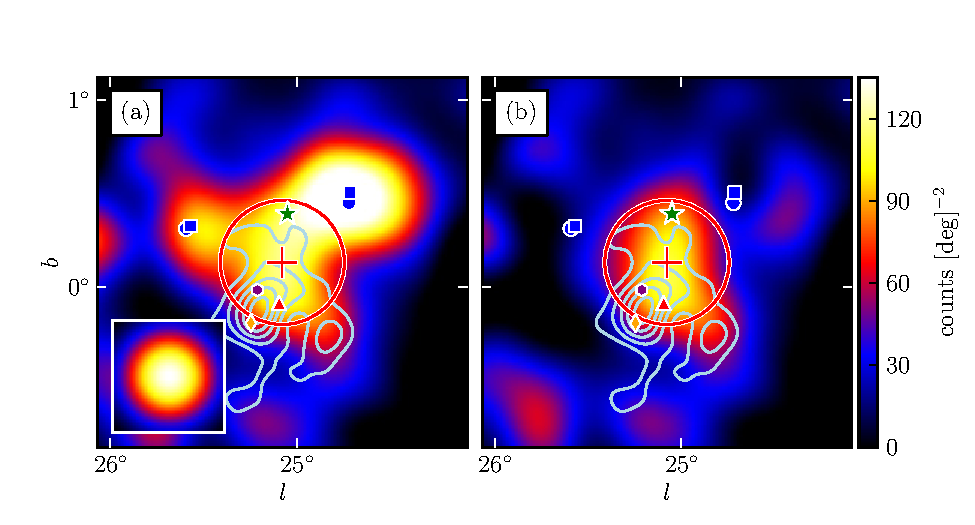
\includegraphics[scale=0.3]{plots/source_HESS_J1837-069_color.pdf}

    \begin{itemize}
      \item Coincident with HESS\,J1837-069
      \item + X-ray pulsar PSR\,J1838$-$0655 
      \item + $\sim 2'$ X-ray PWN 
      \item PWN candidate
      \item Second X-ray PSR + PWN candidate in region
        (but no pulsations)
    \end{itemize}
  \end{columns}
\end{frame}


\begin{frame}{Thank you}
  See text for more details:
  \begin{itemize}
    \item
  \url{https://www-glast.stanford.edu/cgi-prot/pub_download?id=662}
  \end{itemize}

\end{frame}

\end{document}
